\question[15] En la figura \ref{fig:triang_sem05} $\overline{RA}$ es paralelo a $\overline{ET}$ ($\overline{RA}\parallel\overline{ET}$) y la longitud de $RT$ es $21$ unidades.
Calcula la longitud de $\overline{ST}$.
Escribe tu respuesta con un número decimal, redondéala a la centésima más cercana.


\begin{minipage}{\textwidth}
    \begin{minipage}{0.65\textwidth}
        \begin{solutionbox}{8cm}

        \end{solutionbox}
    \end{minipage}\hfill
    \begin{minipage}{0.35\textwidth}
        \begin{figure}[H]
            \centering
            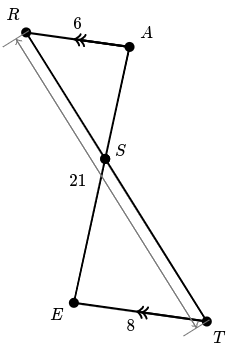
\includegraphics[width =0.9\linewidth ]{Images/triang_sem05}
            \caption{}
            \label{fig:triang_sem05}
        \end{figure}
    \end{minipage}
\end{minipage}